\chapter{Proof of Concept}

\section{Systemübersicht}
Das Proof of Concept beinhaltet die Logik und Kommunikation zwischen dem Gestensensor und der Drohne über die jeweils bestehenden \gls{apiLabel}'s (orange eingefärbter Teil).

Folglich sind die zwei Hauptkomponenten der Umsetzung der \textit{Crazyflie Controller} (\secref{sec:poc:controllerCrazyflie}) und der \textit{Detection Controller} (\secref{sec:poc:controllerDetection}).

\begin{figure}[H]
	\centering
	\includegraphics[width=0.8\textwidth]{figures/system_poc.pdf}
	\caption{System-Überblick: Proof of Concept}
\end{figure}

\subsection{Crazyflie Controller}
\label{sec:poc:controllerCrazyflie}
Der Crazyflie Controller stellt die Verbindung zur Drohne her, über die Steuerkommandos übermittelt werden können.
Dabei stellt das Management der Verbindung den Hauptteil des Codes dieses Controllers dar.
Beim Verbindungsaufbau sowie bei erfolgreicher Verbindung müssen mögliche Fehler-Events abgefangen werden und der Zustand der Verbindung muss von aussen abrufbar sein.
Ansonsten hat der Crazyflie Controller keine Aufgabe.

\subsection{Detection Controller}
\label{sec:poc:controllerDetection}
Der Detection Controller bildet den Kern der Applikation. Er kommuniziert mit dem Leap Motion, erhält die Gesteninformationen, wertet diese abhängig des Zustandes der Steuerung aus und definiert daraus die Kommandos, die via den Crazyflie Controller der Drohne übermittelt werden sollen.
Die ganze Logik der Steuerung befindet sich dementsprechend in diesem Teil.

Um die Auswertung der Gesten abhängig des Zustandes angemessen aufzuteilen, gibt es für jeden Zustand einen eigenen \textit{State Handler}.

\newpage
\subsection{Programm Ablauf}
Folgendes Ablauf-Diagramm soll den systematischen Ablauf des Programmes aufzeigen.
Im Teil \textit{Init} werden die verschiedenen Komponenten verbunden.
Im \textit{Controlling} befindet sich die Steuerung.
Im \textit{Shut down} wird das Programm beendet.

\vspace{7mm}
\begin{figure}[H]
	\centering
	\includegraphics[width=1.0\textwidth]{figures/poc/flowchart_controll.png}
	\vspace{0.7\baselineskip}
	\caption{Ablaufdiagramm: Steuerung}
\end{figure}


\newpage
\subsection{Datei-Struktur}
\begin{wrapfigure}{R}{0.4\textwidth}
	\includegraphics[width=1.0\linewidth]{figures/poc/filestructure.png}
	\caption{Dateistruktur der Umsetzung}
\end{wrapfigure}
%\begin{wrapfigure}{l}{0.4\textwidth}
%	\includegraphics[width=1.0\linewidth]{figures/poc/filestructure.png}
%	\caption{Dateistruktur der Umsetzung}
%\end{wrapfigure}
Die gesamte Umsetzung im Verzeichnis \textit{code} besteht aus drei Modulen und ist wie folgt aufgegliedert:

\subsubsection{Controller}
Die Controller wurden bereits oben erwähnt. Jeder Controller trägt die Verantwortung einer Komponente (Detection via Leap Motion oder Crazyflie).
Nach dem Aufruf eines Controllers übernimmt der Controller die Kommunikation und Verwaltung der zugeordneten Komponente.

Um die Controller schlank zu halten, greifen sie auf Code aus weiteren Modulen (\textit{Piloting} und \textit{StateHandler}) zu.
Um eine Komponente via \gls{apiLabel} zu verwenden, werden oft folgende Schritte benötigt:
Die Verbindung zur Komponente muss aufgebaut werden und kann über verschiedene Parameter konfiguriert werden.
Zudem können diverse Callback-Events registriert werden, die von der Komponente bei bestimmten Ereignissen aufgerufen werden können. Beispiele sind: erfolgreiche Verbindung, Verbindungsunterbruch, Abarbeitung von Daten die zur Verfügung stehen (wie erkannte Gesten vom Leap Motion) usw.

\subsubsection{State Handler}
Jeder Status, in den die Drohne versetzt werden kann, wird durch einen eigenen \textit{StateHandler} abgebildet.
Ein \textit{StateHandler} hat Zugriff auf die Gesteninformationen und wertet diese gemäss den statusabhängigen Möglichkeiten aus.
Wird der Status (\textit{next\_state}) geändert, wird beim nächsten verfügbaren Frame jener \textit{StateHandler} aufgerufen.

In der vorliegenden Umsetzung gibt es die folgenden \textit{StateHandlers}:
\begin{itemize}
	\item \textit{State1InitHandler}
	\item \textit{State2FlightreadyHandler}
	\item \textit{State3FlightHandler}
	\item \textit{State\_ResetHandler}
\end{itemize}
Alle \textit{StateHandler} erben von der \textit{BaseStateHandler}-Klasse, welche die grundsätzlich verfügbaren Variablen definiert (erkannte Gesten, Crazyflie, und den eigenen sowie den nächsten Status).

\subsubsection{Piloting}
Das Modul Piloting beinhaltet allgemeine, steuerspezifische Konfigurationen.
Dazu gehört die Verknüpfung zwischen Status-Nummer, Status-Bezeichnung und dem jeweiligen StateHandler, sowie verschiedene Flugparameter (z.B.: maximale Power).

Nebst der Konfiguration beinhaltet das \textit{Piloting}-Modul einen \textit{LeapListener}, der die notwendigen Callbacks für den Leap Motion Sensor registriert. Darunter die Funktion \textit{on\_frame()}, die bei jedem erkannten Frame aufgerufen wird.
Es befindet sich aber kein Status spezifischer Code im \textit{Piloting}.

\subsubsection{main.py}
Das \textit{main.py} File dient zum Starten des Programmes. Es erstellt die Controller und überprüft auf eine gewünschte Programmbeendigung. Somit entspricht das \textit{main} File dem Root-File.


\section{Implementation der Drohne}
\subsection{Verbindung zur Drohne herstellen}
Die Crazyflie Library wird wie folgt eingebunden:
\begin{lstlisting}[style=lstStyleCpp]
sys.path.append("lib/crazyflie")
import cflib
from cflib.crazyflie import Crazyflie
\end{lstlisting}

Mit dem \textit{Scannen} wird der Link der Drohne gefunden und die Verbindung kann hergestellt werden:
\begin{lstlisting}[style=lstStyleCpp]
available = cflib.crtp.scan_interfaces()
#link_uri = available[0][0]
link_uri = 'radio://0/80/250K'

cf = Crazyflie()

self.cf.connected.add_callback(self._connected)
self.cf.disconnected.add_callback(self._disconnected)
self.cf.connection_failed.add_callback(self._connection_failed)
self.cf.connection_lost.add_callback(self._connection_lost)

# connect to drone
self.cf.open_link(link_uri)
\end{lstlisting}

Da \textit{scan\_interfaces} oft auch Störsignale zurückliefert, wurde der Kommunikationslink statisch auf "`radio://0/80/250K"' codiert.

Der vollständige Code kann unter \href{https://github.com/MrJack91/droneGestures/blob/master/code/Controller/CrazyflieController.py}{/code/Controller/DetectionController.py} eingesehen werden.

\subsection{Steuerkommando übermitteln}
Wenn die Drohne erfolgreich verbunden wurde, kann ein Steuerbefehl folgendermassen abgesetzt werden:

\begin{lstlisting}[style=lstStyleCpp]
cf.commander.send_setpoint(roll, pitch, yaw, thrust)
\end{lstlisting}

Dabei müssen die Vorzeichen sorgfältig gesetzt werden, sonst erfolgen Teile der Steuerung spiegelverkehrt.


\section{Implementation der Gestenerkennung}
Wie in \secref{subsec:leapmotion:api} beschrieben, kann der Leap Motion sehr viele Informationen erkennen und zurückliefern.
Für die geplante Gestensteuerung reicht es jedoch aus, wenn die Richtungsvektoren von Hand-Objekten innerhalb einzelner Frames ausgewertet werden.
Es müssen keine Gesten über mehrere Frames erkannt werden. (Der Leap Motion unterstützt auch die Erkennung von grundlegenden Gesten über mehrere Frames. Es können Callbacks auf bestimmte Gesten definiert werden, in denen bereits die Aktion ausgeführt werden kann. Dies wird für die vorliegende Umsetzung, wie erwähnt, nicht benötigt.)

\subsection{Leap anbinden}
Die Leap Motion Library wird auf OS X folgendermassen eingebunden:
\begin{lstlisting}[style=lstStyleCpp]
# lib (for os x)
src_dir = os.path.dirname(inspect.getfile(inspect.currentframe()))
lib_dir = os.path.abspath(os.path.join(src_dir, '../lib/leap'))
sys.path.insert(0, lib_dir)
\end{lstlisting}

Anschliessend kann ein Leap-Controller erstellt werden, welchem ein Listener-Objekt hinzugefügt werden kann:
\begin{lstlisting}[style=lstStyleCpp]
# register callback object who contains the on_frame() method
controller = Leap.Controller()
controller.add_listener(LeapListener.LeapListener())
\end{lstlisting}

Der vollständige Code kann unter \href{https://github.com/MrJack91/droneGestures/blob/master/code/Controller/DetectionController.py}{/code/Controller/DetectionController.py} eingesehen werden.

\subsection{Benötigte Gesten erkennen}
Grundsätzlich wird jedes Frame auf vorhandene Hand-Objekte geprüft.
Falls genau ein Hand-Objekt vorhanden ist, werden diese Daten ausgewertet. Wenn mehrere Hände erkannt werden, wird die Steuerung in den Reset-Zustand zurückgesetzt und die Initialisierung beginnt von vorne.

Für die Logik des Init-Prozesses, vom \textit{Reset-} bis zum \textit{Flug-Zustand (Z3)}, muss lediglich die Faust erkannt werden.
Der Wert \textit{grab\_strength} enthält einen Wert zwischen null und eins, wobei null einer offenen Hand und eins einer Faust entspricht.
Dieser Wert kann wie folgt abgerufen werden:

\begin{lstlisting}[style=lstStyleCpp]
frame.hand[0].grab_strength
\end{lstlisting}

Im \textit{Flug-Zustand (Z3)} werden verschiedene Richtungsvektoren der erkannten Hand abgerufen:

\begin{lstlisting}[style=lstStyleCpp]
# Thrust (Drehanzahl / Höhe): absolut height of the hand palm
thrust = frame.hand[0].palm_position.y

# Direction vector of the hand: from hand palm to finger (pitch -> Neigung; yaw -> Drehung / Gieren)
pitch = frame.hand[0].direction.pitch
yaw = frame.hand[0].direction.yaw

# Direction of the normal vector, to measure the roll (Rolle)
roll = frame.hand[0].palm_normal.roll
\end{lstlisting}

\begin{itemize}
	\item \textit{Zeile 2:}
	Mit \textit{palm\_position} kann die Position des Handballen gelesen werden.
	Der Y-Wert entspricht der Höhe, welche für den Thrust verwendet wird.
	Der effektive Thrust muss abhängig von der Ausgangsposition der Hand berechnet werden.

	\item \textit{Zeile 5 und 6:}
	\textit{Direction} liefert Richtungsvektoren ausgehend aus der Handballe in Richtung der Finger. So wird die Pitch (Neigung) und der Yaw (Drehung / Gieren) gelesen.

	\item \textit{Zeile 9:}
	Der \textit{palm\_normal} Vektor steht im rechten Winkel zur Handballen. Daraus kann der Roll (Rolle) definiert werden.
\end{itemize}

Alle Winkel werden in Radian gemessen und müssen für die Crazyflie in Grad umgewandelt werden.

\subsection{Testen der Gestensteuerung}
Gemäss der Aufgabenstellung soll ein Testen der Gestensteuerung ohne fliegende Drohne möglich sein.
Dazu wurde ein Debug-Parameter eingeführt.
Ist der gesetzt, wird die Drohne nicht verbunden, sondern die Gestensteuerung kann eigenständig getestet werden.

Jener Debug-Parameter findet sich im Main-File (\href{https://github.com/MrJack91/droneGestures/blob/master/code/main.py}{/code/main.py}) und kann dort gesetzt werden.



\section{Anpassungen am Konzept}
\label{sec:poc:conceptChanges}
Die ursprüngliche Steuerung (gemäss \secref{sec:concept:stateoverview}) wurde während der Umsetzung optimiert.\\
Das Zustands-Diagramm wurde wie folgt angepasst:
\begin{figure}[H]
	\centering
	\includegraphics[width=1.0\textwidth]{figures/concept/state-diagram-2.pdf}
	\caption{Zustands-Diagramm: optimierte Steuerlogik}
\end{figure}

Folgend werden die durchgeführten Änderungen erläutert und begründet.

\subsection{"'Z4: unkontrolliert"' entfernt}
Ein neues Bedürfnis aus Perspektive des Piloten wurde erkannt: Die Drohne soll bei kritischen Flugsituationen in der Lage sein möglichst rasch gestoppt zu werden, resp. die Rotoren auszuschalten.
So kann Schaden an den Rotoren vermieden werden, welche am häufigsten ersetzt werden müssen, da sich diese in Bewegung befinden und bei einer Kollision eine grössere Kraft darauf auswirkt.
Zudem wird auch die Möglichkeit an Schäden durch drehende Rotoren gehemmt, was aber bei dieser Drohnengrösse eher ein theoretisches Risiko darstellt.
In diesem Fall wird ein unkontrollierter Absturz in Kauf genommen.

Gleichzeitig zeigten diverse Testflüge, dass die Verbindung zur Drohne, sowie auch die zum Leap Motion, sehr stabil läuft und daher keine unerwartete Unterbrüche zu überbrücken sind.

Da in kritischen Flugsituationen meist die Reaktionszeit des Piloten eine grosse Rolle spielt, muss ein Rotorenstop möglichst intuitiv erfolgen.
Daher wurde die Steuerung so angepasst, dass die Rotoren stoppen, sobald eine Faust erkannt wird oder die Hand nicht mehr erkannt wird.

Der Zustand \textit{Z4: unkontrolliert} wurde daher entfernt.
Diese Anpassung hat sich bei mehreren Testflügen bereits bewährt.

\subsection{Init-Prozess: "`Reset"' hinzugefügt}
Ein eher kleines, aber bereits im Konzept vernachlässigtes Problem einer Gestensteuerung, stellt die zwar korrekte Erkennung von Gesten, aber nicht beabsichtigte Ausführung davon dar.
Wenn die Applikation initialisiert wird, soll keine nicht-gewollte  Geste die Drohne in die Luft bringen können.
Denn ansonsten wird entweder direkt anschliessend keine Hand mehr erkannt, was zum Absturz führt, oder es folgen weitere nicht bewusste Kommandos, die gefährlich für die Drohne und das Umfeld sein können.

Aufgrund dieser Gefahr wurde die Sicherheit des Init-Prozesses mit einem weiteren Pseudo-Zustand erweitert: dem \textit{Reset-Zustand}.

Vor dem \textit{Init-Zustand (Z1)} befindet sich die Drohne im \textit{Reset-Zustand}. Der Zustandswechsel in den \textit{Init-Zustand (Z1)} kann erst erfolgen, wenn nacheinander eine Faust und eine offene Hand erkannt werden.
Damit wird vermieden, dass nach der Landung ein Öffnen der Hand bereits als neue Initialisierung des nächsten Fluges ausgeführt wird und die Drohne beim unvorsichtigen Entfernen der Hand bereits los fliegt.
Zudem hilft dies, generell nicht gewollte Gesten, die ein Steuerkommando zur Folge hätten, zu ignorieren.

Da trotz der erwähnten Vorsichtsmassnahme noch nicht genügend gewährleistet werden kann, dass die Geste wirklich einen Start auslöst, wird erst dann in den \textit{flugbereiten Zustand (Z2)} gewechselt, wenn mindestens 2 Sekunden lang eine Faust-Geste erkannt wird.

Bei jedem Not-Abbruch, egal in welchem Zustand sich die Steuerung befindet, wird die Steuerung wiederum in den Reset-Zustand versetzt.

Mit Hilfe dieser Anpassungen hat sich bis jetzt der gesamte Init-Prozess als sicher erwiesen.
Unabsichtliche Steuerungen wurden seither konsequent ignoriert.

\subsection{Anpassung vom Zustand "`Z2: flugbereit"'}
Ursprünglich war geplant, dass der Zustandswechsel zwischen \textit{flugbereitem Zustand (Z2)} und \textit{Flug-Zustand (Z3)} abhängig davon ist, ob sich die Drohne in der Luft oder auf dem Boden befindet.
Dies ist jedoch mit den Sensoren schwierig zu erkennen und bringt für die implementierte Steuerung keinen Vorteil.

Daher wurde der Wechsel vom \textit{flugbereiten Zustand (Z2)} in den \textit{Flug-Zustand (Z3)} neu definiert.
Der Wechsel erfolgt sobald eine offene Hand (innerhalb akzeptierter Höhe) erkannt wird.
Somit erzwingt der neue \textit{Flug-Zustand (Z3)} nicht explizit, dass sich die Drohne in der Luft befindet, jedoch die Steuerung (Gestenerkennung inklusive Befehlsübermittlung) entspricht den Möglichkeiten, die der Pilot in der Luft zur Verfügung hat.



\section{Mögliche Erweiterungen}
\label{sec:extensions}
Bereits bei der Planung der Arbeit wurden mögliche Erweiterungen in Form von Prioritäten, die bei genügen Zeit umgesetzt werden sollen, eingeplant.
Während der Entwicklung wurden weitere Ideen gesammelt.
Eine Übersicht möglicher Erweiterungen wird im Folgenden kurz zusammengefasst.

\subsection{Hilfstexte in der Konsole}
Um die Anwendung für Dritte zu vereinfachen, sollte in der Konsole, nebst dem aktuellen Zustand der Steuerung, auch noch der nächste notwendige Schritt angezeigt werden.
Zudem könnte zu Beginn eine allgemeine Steueranleitung ausgegeben werden.
Falls Probleme zwischen der Steuerung und einem externen System auftreten, sollten nebst der Fehlermeldung auch noch Lösungsmöglichkeiten angezeigt werden.

\subsection{Sound Unterstützung}
Zum jetzigen Zeitpunkt wird ein Zustandswechsel der Steuerung in der Konsole ausgegeben.
Somit muss während der Initialisierung ständig einen Blick auf den Konsolen-Output geworfen werden.
Um dies zu umgehen, könnte bei jedem erfolgreichen Zustandswechsel ein Ton abgespielt werden.
Falls die Steuerung zurück in den \textit{Reset-Zustand} fällt, soll ein weiterer Ton den Benutzer über den Wechsel informieren.

\subsection{User Interface mit mehr Informationen}
Momentan zeigt die Anwendung lediglich den Zustand der Steuerung an.
Weitere Informationen zu den externen Systemen, wie der Akkustand, die Verbindungsqualität oder zusätzliche Debug-Informationen könnten regelmässig (z.b. alle 5 Sekunden) ausgegeben werden.
Alternativ dem Konsolen-Output könnte auch ein \gls{guiLabel} verwendet werden.
So wären die Informationen übersichtlicher und einfacher dargestellt.

\subsection{Flug Improvements / einfachere Steuerung}
Um die Steuerung zu vereinfachen, könnten aktuelle Gesteninformationen mit vorgängigen Gesten und dem Zustand der Drohne kombiniert werden. Daraus kann dann ein intelligentes Steuerkommando berechnet werden.
Beispiele dazu wäre das Abschwächen von starken Steueranweisungen oder das automatische Stabilisieren der Drohne, wenn die Hand vertikal ruhig gehalten wird.

\newpage
\subsection{Automatische Flugmanöver}
In der ursprünglichen Planung wurden automatische Flugmanöver erwähnt.
Aufgrund eingeschränkten zeitlichen Ressourcen für die Umsetzung, wurden solche Manöver bereits vor Projektbeginn aus der Aufgabenstellung wieder entfernt.

Es folgt eine Liste mit möglichen automatischen Flugmanövern:
\begin{itemize}
	\item \textbf{Stabilisieren:}
	Via einer Gestenbewegung soll die Drohne in einen Schwebeflug versetzt werden. Dabei haltet die Drohne möglichst genau die Position in der Luft.

	\item \textbf{Landung:}
	Die Drohne soll automatisch, kontrolliert und sicher landen können. Die Landung kann entweder durch eine Geste oder bei kritischen Situationen wie einer Kommunikationsstörung ausgelöst werden.
	Da das Umfeld der Drohne nicht bekannt ist, wäre eine stabile, langsame Senkung der Höhe mit Hilfe des Gyrometers und des Accelerometers am Besten geeignet.

	\item \textbf{Kunstflug:}
	Unter Kunstflugmanöver sind spezielle Flugformen gemeint. Zum Beispiel das Abfliegen eines Quadrates oder die Ausführung eines Überschlages etc.

	\item \textbf{Flucht:}
	Fluchtmanöver sollten das Einfangen oder Abschiessen der Drohne verhindern, indem schnelle, sprunghafte Bewegungen in drei Dimensionen ausgeführt werden.
	Solche Fluchtmanöver könnten anhand von externen Sensoren ausgelöst werden.
	Dabei muss überprüft werden, ob in der Richtung in der das Manöver ausgeführt werden soll, auch genügend freien Platz vorhanden ist.
	Dazu sind weitere Sensoren wie Distanzmesser oder Kameras notwendig.

\end{itemize}


\newpage
\section{Diagramme}

\subsection{Ablauf - Sequenz-Diagramme}
Nachstehend werden einzelne Sequenzen mit Hilfe eines Sequenz-Diagrammes genauer aufgezeigt.

\subsubsection{Programmstart}
Die ersten zwei Diagramme zeigen den Ablauf der Initialisierung des Controllers bis zur Abarbeitung des Frames vom Leap Motion auf.
\begin{figure}[H]
	\centering
	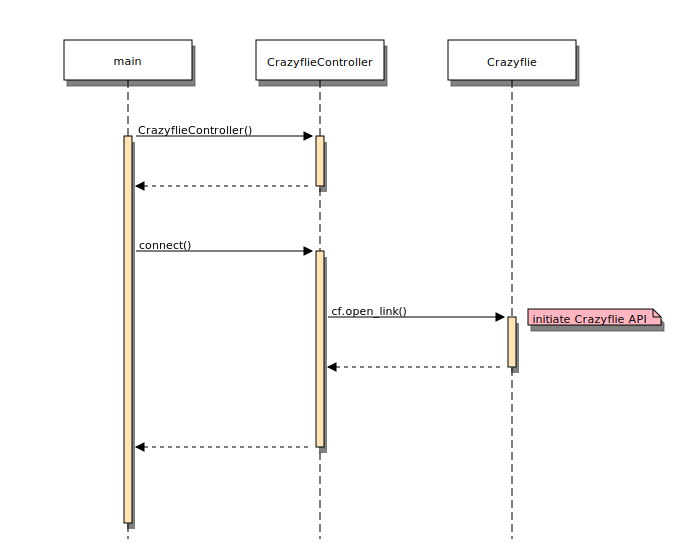
\includegraphics[width=1.0\textwidth]{figures/poc/seq_dia_crazyflie.png}
	\caption{Sequenz-Diagramm - Initialisierung der Crazyflie}
\end{figure}

%\begin{figure}
%	\centering
%	\def\svgwidth{\columnwidth}
%	\input{figures/poc/seq_dia_detection.pdf}
%\end{figure}


\begin{sidewaysfigure}[ht]
	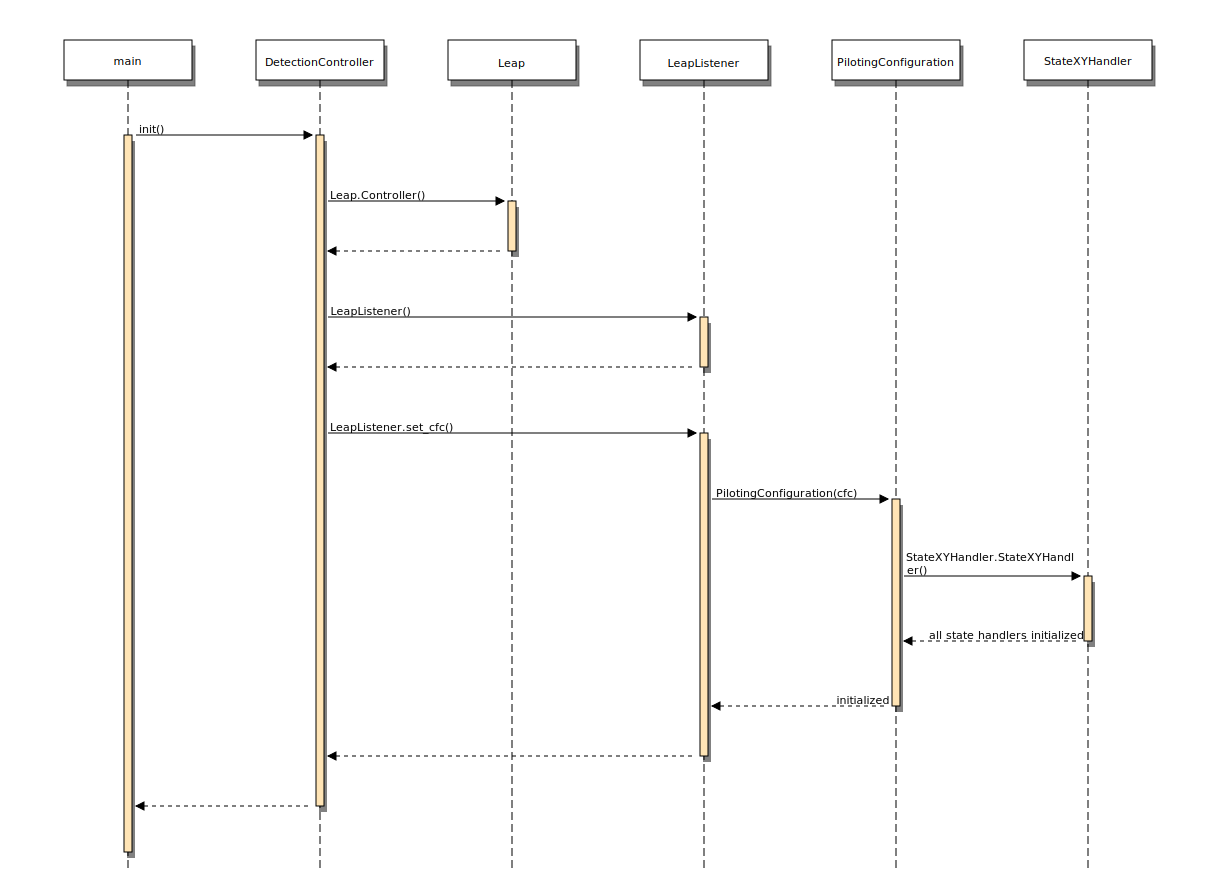
\includegraphics[width=1.0\textwidth]{figures/poc/seq_dia_detection_part1.png}
	\caption{Sequenz-Diagramm - Initialisierung des Leap Motions}
\end{sidewaysfigure}

\begin{sidewaysfigure}[ht]
	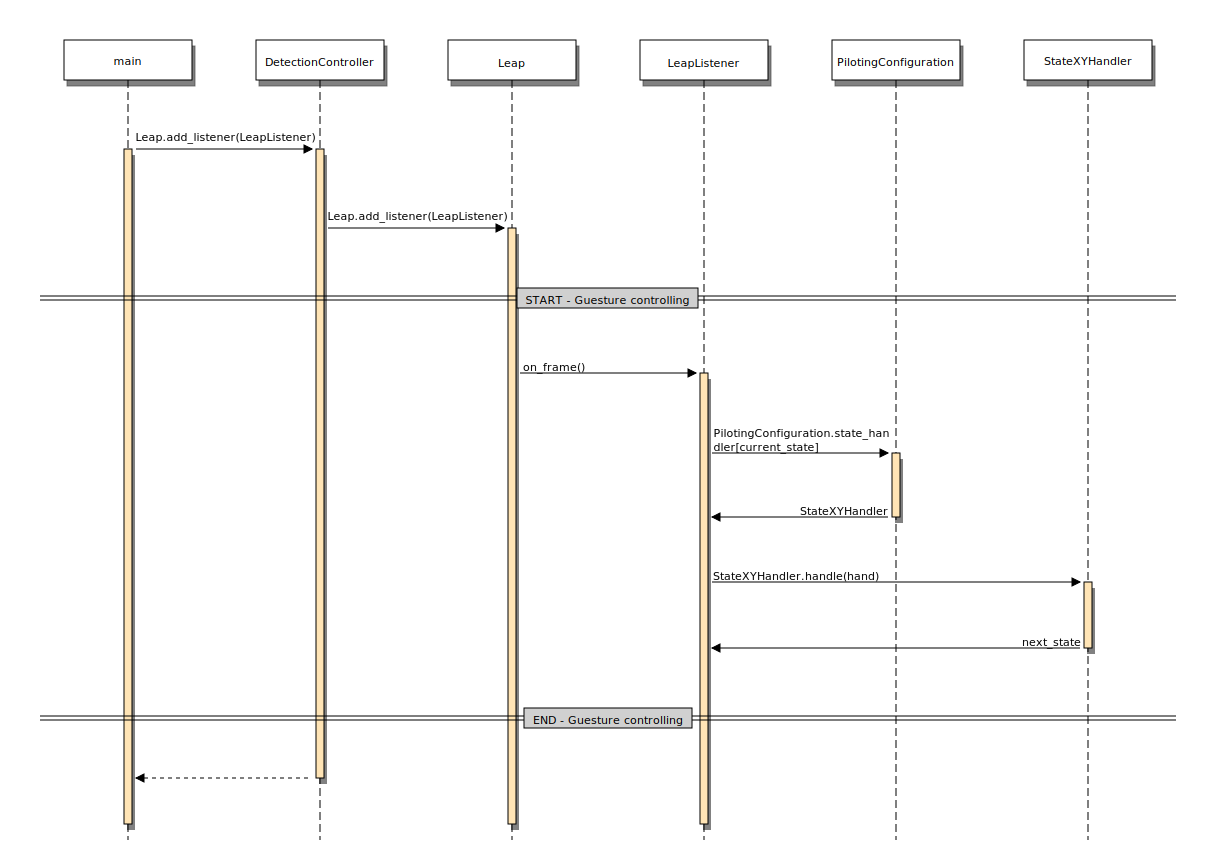
\includegraphics[width=1.0\textwidth]{figures/poc/seq_dia_detection_part2.png}
	\caption{Sequenz-Diagramm - Gestenerkennung und Ausführung der allgemeinen Steuerung}
\end{sidewaysfigure}

%\begin{figure}[H]
%	\centering
%	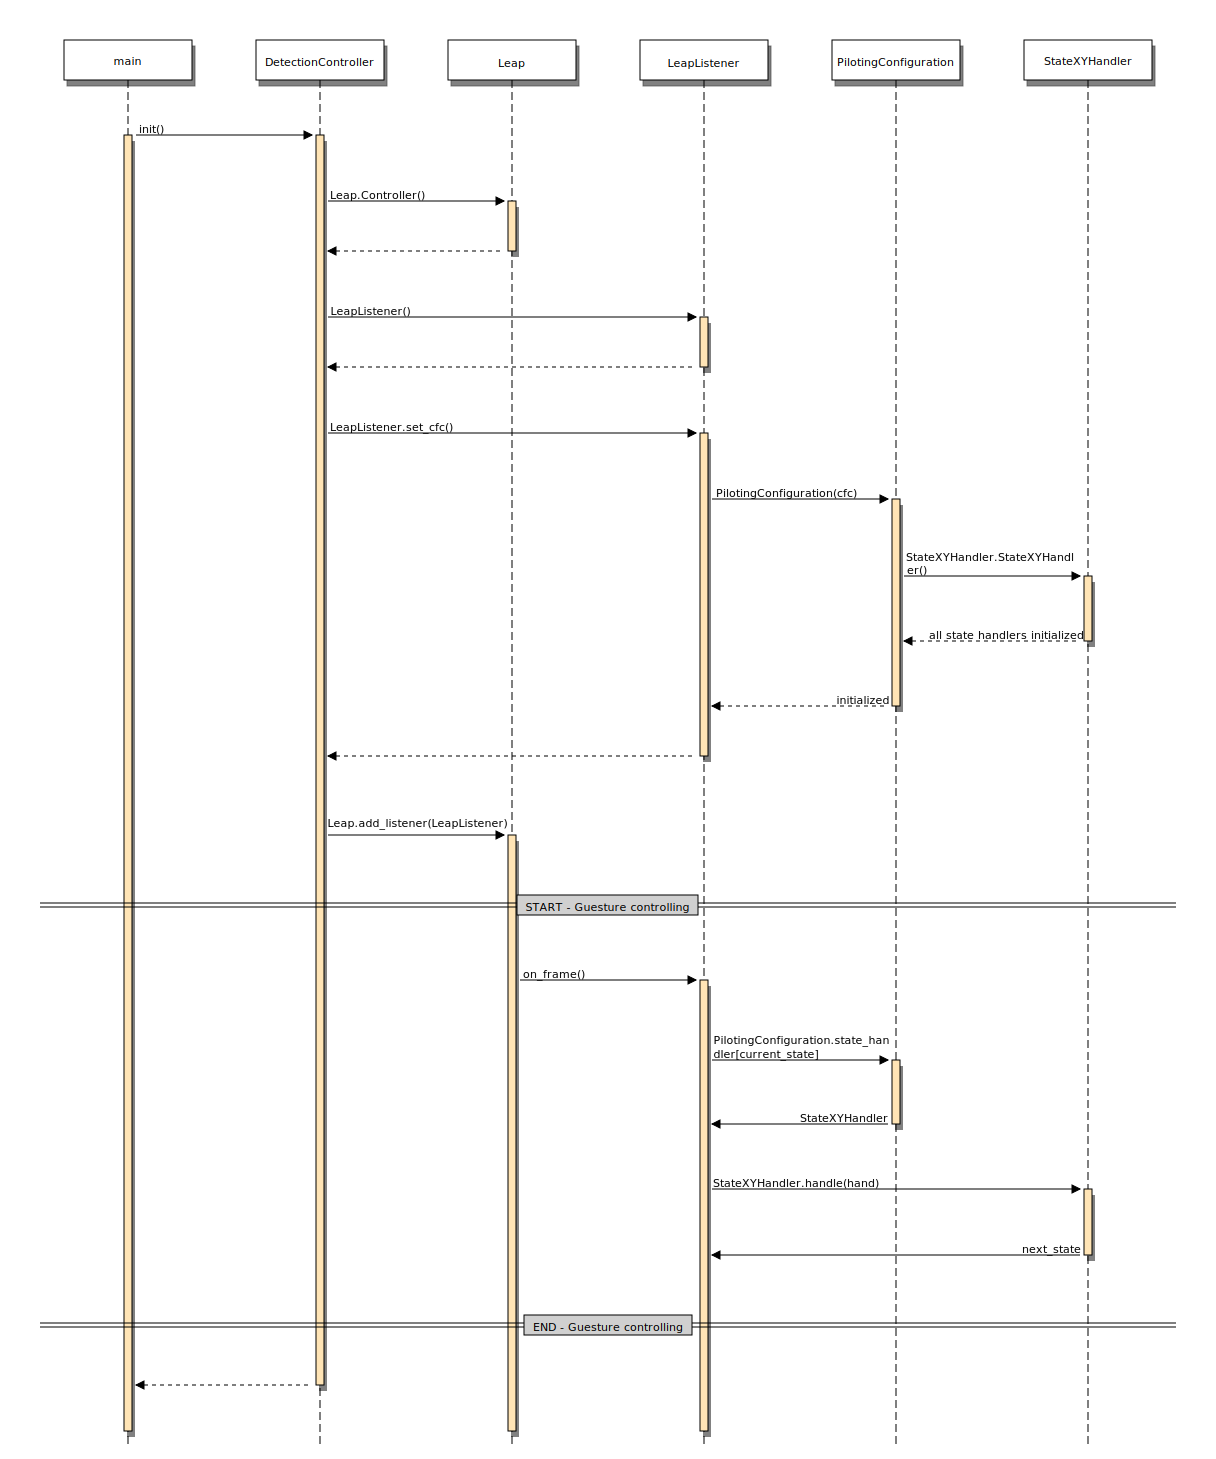
\includegraphics[width=1.0\textwidth]{figures/poc/seq_dia_detection.png}
%	\caption{Sequenz-Diagramm - Initialisierung und Ablauf des Leap Motions}
%\end{figure}

\clearpage
\subsection{Programmbeendung}
Dieses Diagramm zeigt die korrekte Beendigung des Programmes auf.

\begin{figure}[H]
	\centering
	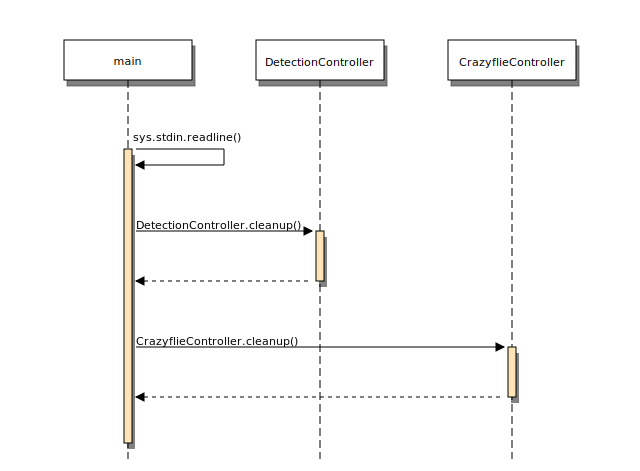
\includegraphics[width=1.0\textwidth]{figures/poc/seq_dia_shutdown.png}
	\caption{Sequenz-Diagramm - Shutdown}
\end{figure}


\subsection{UML}
Folgende \gls{umlLabel}'s zeigen die wichtigen Klassen pro Modul auf. Dies soll einen vereinfachten Blick auf die Umsetzung ermöglichen.

\begin{figure}[H]
	\centering
	\includegraphics[width=0.5\textwidth]{figures/poc/uml/controller.png}
	\caption{UML - \textit{Controller} Modul}
\end{figure}

\begin{figure}[H]
	\centering
	\includegraphics[width=0.81\textwidth]{figures/poc/uml/piloting.png}
	\caption{UML - \textit{Piloting} Modul}
\end{figure}

\begin{figure}[H]
	\centering
	\includegraphics[width=1.0\textwidth]{figures/poc/uml/stateHandler.png}
	\caption{UML - \textit{StateHandler} Modul}
\end{figure}
